
\documentclass[11pt]{article}

\usepackage{amsmath,amssymb}
\usepackage[margin=1in]{geometry}
\usepackage{setspace}
\usepackage{pgfplots}
\usepackage{array}

\pgfplotsset{compat=1.18}

\setstretch{1.05}

\begin{document}

\begin{center}
    {\large \textbf{MATH4041/MCSC6120 Assignment 1}}\\
    \vspace{2mm}
    \textbf{Glucose Control, Part 1}\\
    \vspace{1mm}
    Logan Bostelmann
\end{center}

\section*{1. Derivation of the Two-Degree-of-Freedom Model}

We begin with the glucose control model introduced in lecture,
which consists of an integral equation and a differential equation:
\begin{equation}
u
=
\alpha v
+
\beta
\int_{-\infty}^{t}
\lambda e^{-\lambda(t-t')}v(t')\,dt',
\end{equation}
and
\begin{equation}
\dot v
=
-\gamma v-\delta u(v+\bar v)+F(t).
\end{equation}

Our goal is to eliminate the integral so that the model can be
expressed as a system of two ordinary differential equations.
To do this, we first differentiate the equation for \(u\)
with respect to time:
\begin{align}
\dot u
&=
\alpha\dot v
+
\beta\lambda
\frac{d}{dt}
\left(
\int_{-\infty}^{t}
e^{-\lambda(t-t')}v(t')\,dt'
\right).
\end{align}

Since the upper limit of integration depends on \(t\),
we apply Leibniz's rule:
\begin{align}
\dot u
&=
\alpha\dot v
+
\beta\lambda
\left(
v(t)
-
\lambda
\int_{-\infty}^{t}
e^{-\lambda(t-t')}v(t')\,dt'
\right)\\
&=
\alpha\dot v
+
\beta\lambda v
-
\lambda
\left(
\beta
\int_{-\infty}^{t}
\lambda e^{-\lambda(t-t')}v(t')\,dt'
\right).
\end{align}

Notice that the remaining integral is the same one that
appears in our original equation for \(u\). Rearranging
that equation gives:
\begin{equation}
\beta
\int_{-\infty}^{t}
\lambda e^{-\lambda(t-t')}v(t')\,dt'
=
u-\alpha v.
\end{equation}

We can now substitute this expression into our derivative:
\begin{align}
\dot u
&=
\alpha\dot v
+
\beta\lambda v
-
\lambda(u-\alpha v)\\
&=
\alpha\dot v
+
\lambda(\alpha+\beta)v
-
\lambda u.
\end{align}

Finally, we introduce the notation:
\begin{equation}
\dot v=f(u,v).
\end{equation}

This allows us to express the original model entirely in
terms of two differential equations:
\begin{equation}
\boxed{
\begin{aligned}
\dot u&=-\lambda u+\lambda(\alpha+\beta)v+\alpha f(u,v),\\
\dot v&=-\gamma v-\delta u(v+\bar v)+F(t).
\end{aligned}}
\end{equation}

We have therefore obtained the required two-degree-of-freedom
ODE system without the integral term.

\section*{2. Scaling the Variables}

We now want to simplify the system by introducing dimensionless
variables, reducing the number of parameters appearing in
the equations.

Recall the system obtained in Question 1:
\begin{equation}
\begin{aligned}
\dot u&=-\lambda u+\lambda(\alpha+\beta)v+\alpha f(u,v),\\
\dot v&=-\gamma v-\delta u(v+\bar v)+F(t).
\end{aligned}
\end{equation}

Following the scaling approach from lecture, we introduce:
\begin{equation}
t=\tilde t\,t',
\qquad
u=\tilde u\,u',
\qquad
v=\bar v\,v'.
\end{equation}

Because time is also being rescaled, we must account for
this when transforming the derivatives:
\begin{equation}
\dot u
=
\frac{\tilde u}{\tilde t}\frac{du'}{dt'},
\qquad
\dot v
=
\frac{\bar v}{\tilde t}\frac{dv'}{dt'}.
\end{equation}

Here, \(f'(u',v')\) represents the original dimensional
function \(f\) evaluated using the scaled variables.

Substituting the new variables into both equations gives:
\begin{align}
\frac{\tilde u}{\tilde t}\frac{du'}{dt'}
&=
-\lambda\tilde u u'
+
\lambda(\alpha+\beta)\bar v v'
+
\alpha f'(u',v'),
\\
\frac{\bar v}{\tilde t}\frac{dv'}{dt'}
&=
-\gamma\bar v v'
-
\delta\tilde u u'(\bar v v'+\bar v)
+
F(t).
\end{align}

Next, we isolate the derivatives by dividing through
by their respective coefficients:
\begin{align}
\frac{du'}{dt'}
&=
-(\lambda\tilde t)u'
+
\left(
\frac{\lambda\bar v\tilde t}{\tilde u}
\right)(\alpha+\beta)v'
+
\left(
\frac{\alpha\tilde t}{\tilde u}
\right)f'(u',v'),
\\
\frac{dv'}{dt'}
&=
-(\gamma\tilde t)v'
-
(\delta\tilde u\tilde t)u'(v'+1)
+
\frac{\tilde t}{\bar v}F(t).
\end{align}

To make the second equation simpler, we choose the time
and \(u\)-scales such that:
\begin{equation}
\gamma\tilde t=1,
\qquad
\delta\tilde u\tilde t=1.
\end{equation}

This gives:
\begin{equation}
\boxed{
\tilde t=\frac{1}{\gamma},
\qquad
\tilde u=\frac{1}{\delta\tilde t}
=\frac{\gamma}{\delta}.
}
\end{equation}

We also introduce the scaled input parameter:
\begin{equation}
\boxed{
G=\frac{\tilde t}{\bar v}F(t).
}
\end{equation}

With these choices, the system becomes:
\begin{align}
\frac{du'}{dt'}
&=
-\frac{\lambda}{\gamma}u'
+
\frac{\lambda\delta\bar v}{\gamma^2}
(\alpha+\beta)v'
+
\frac{\alpha\delta}{\gamma^2}f'(u',v'),
\\
\frac{dv'}{dt'}
&=
-v'-u'(v'+1)+G.
\end{align}

We can simplify the notation further by defining
three new parameters:
\begin{equation}
\boxed{
a=\frac{\lambda}{\gamma},
\qquad
b=\frac{\lambda\delta\bar v}{\gamma^2}(\alpha+\beta),
\qquad
c=\frac{\alpha\delta}{\gamma^2}.
}
\end{equation}

Using these definitions, the dimensionless system
can be written more compactly as:
\begin{equation}
\boxed{
\begin{aligned}
\frac{du'}{dt'}&=-au'+bv'+cf'(u',v'),\\
\frac{dv'}{dt'}&=-v'-u'(v'+1)+G.
\end{aligned}}
\end{equation}

This completes the scaling process, leaving us with
a simpler system involving the reduced parameters
\(a\), \(b\), \(c\), and the input \(G\).

\section*{3. Equilibrium Solutions}

To determine the equilibrium solutions, we set both
time derivatives equal to zero. Since our equations
are now dimensionless, we can drop the primes
for simplicity.

The equilibrium conditions are:
\begin{equation}
\boxed{
\begin{aligned}
-au+bv&=0,\\
-v-u(v+1)+G&=0.
\end{aligned}}
\end{equation}

At equilibrium, \(f(u,v)=0\) because it represents
the \(v\)-equation, whose derivative must also vanish.

We begin by solving the first equation for \(u\):
\begin{equation}
-au+bv=0.
\end{equation}

Rearranging gives:
\begin{equation}
\boxed{
u^*=\frac{b}{a}v^*.
}
\end{equation}

We then substitute this relationship into the second
equilibrium equation:
\begin{equation}
-v-\frac{b}{a}v(v+1)+G=0.
\end{equation}

Expanding and collecting terms:
\begin{align}
-\frac{b}{a}v^2-\frac{b}{a}v-v+G&=0,\\
v^2+
\left(1+\frac{a}{b}\right)v
-\frac{a}{b}G&=0.
\end{align}

This is a quadratic equation in \(v\), so applying
the quadratic formula gives:
\begin{equation}
\boxed{
v^*
=
-\frac{1}{2}
\left(1+\frac{a}{b}\right)
\pm
\frac{1}{2}
\sqrt{
\left(1+\frac{a}{b}\right)^2
+
\frac{4a}{b}G
}.
}
\end{equation}

The number of real equilibrium solutions depends on
the expression inside the square root. In particular,
the two solutions coincide when:
\begin{equation}
\left(1+\frac{a}{b}\right)^2
+
\frac{4a}{b}G=0.
\end{equation}

Solving this equation for \(G\) gives the critical
saddle-node value:
\begin{equation}
\boxed{
G_{\mathrm{SN}}
=
-\frac{b}{4a}
\left(1+\frac{a}{b}\right)^2.
}
\end{equation}

Assuming \(a>0\) and \(b>0\), this critical value
separates the three possible cases. For
\(G<G_{\mathrm{SN}}\), there are no real equilibria.
At \(G=G_{\mathrm{SN}}\), the two solutions merge
into one, while for \(G>G_{\mathrm{SN}}\), two
distinct real equilibria exist.

We can summarize these results in the following table:

\begin{center}
\renewcommand{\arraystretch}{1.8}
\small
\begin{tabular}{|c|c|p{8.1cm}|}
\hline
\multicolumn{3}{|c|}{
\textbf{Equilibrium Solutions as a Result of \(G\)}
}\\
\hline
\textbf{Value of \(G\)}
&
\textbf{Number of Solutions}
&
\centering\arraybackslash
\textbf{Equilibrium Solution(s)}
\\
\hline
\(G<G_{\mathrm{SN}}\)
&
Zero
&
N/a
\\
\hline
\(G=G_{\mathrm{SN}}\)
&
One
&
\(\displaystyle
(u^*,v^*)=
\left(
\frac{b}{a}v^*,
-\frac12\left(1+\frac{a}{b}\right)
\right)
\)
\\
\hline
\(G>G_{\mathrm{SN}}\)
&
Two
&
\(\displaystyle
(u^*,v^*)=
\left(
\frac{b}{a}v^*,
-\frac12\left(1+\frac{a}{b}\right)
\pm
\frac12
\sqrt{
\left(1+\frac{a}{b}\right)^2+
\frac{4a}{b}G
}
\right)
\)
\\
\hline
\end{tabular}
\end{center}

To visualize these results, we can sketch the equilibrium
branch against the input parameter \(G\). The curve
illustrates how the two equilibrium solutions meet at
the saddle-node point.

\begin{center}
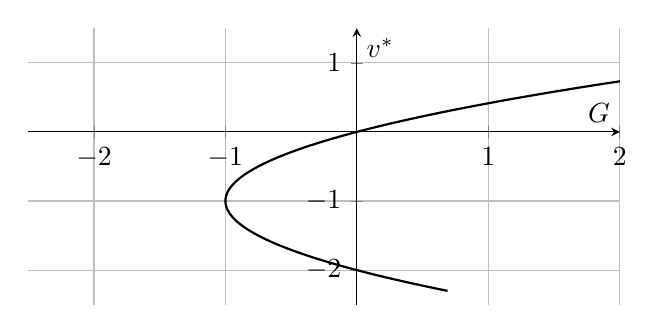
\begin{tikzpicture}
\begin{axis}[
    width=0.75\textwidth,
    height=0.42\textwidth,
    xlabel={$G$},
    ylabel={$v^*$},
    axis lines=middle,
    xmin=-2.5,
    xmax=2.0,
    ymin=-2.5,
    ymax=1.5,
    samples=150,
    domain=-2.3:1.5,
    grid=major
]

\addplot[
    thick
]
({x + x*(x+1)}, {x});

\end{axis}
\end{tikzpicture}
\end{center}

As shown in the sketch, the equilibrium branch bends
at the critical value \(G_{\mathrm{SN}}\). This is
where the two real equilibrium solutions coincide,
illustrating the saddle-node behaviour of the model.

\end{document}
